\chapter{Estado del arte}
En este capítulo se exponen los principales temas de interés para la realización de este trabajo, las investigaciones realizadas sobre la TPV y NF-TPV (termofotovoltaica de campo cercano) y el marco teórico sobre las diferentes maneras que se transmite el calor.

\section{Termo-fotovoltaica}
%%%%%%%%%%%%%%   THERMO PHOTOVOLTAICA       %%%%%%%%%%%%%
Un generador termo-fotovoltaico(TPV) se basa en la conversión de energía calorífica en energía eléctrica mediante el efecto fotovoltaico a través una célula termo-fotovoltaica sin requerir ninguna parte móvil, conocido este tipo de sistemas de generación como motores pasivos de calor, como se representa de una manera sencilla en la figura \ref{fig:TPV_Subsistema}.
\begin{figure}[H]
	\centering
	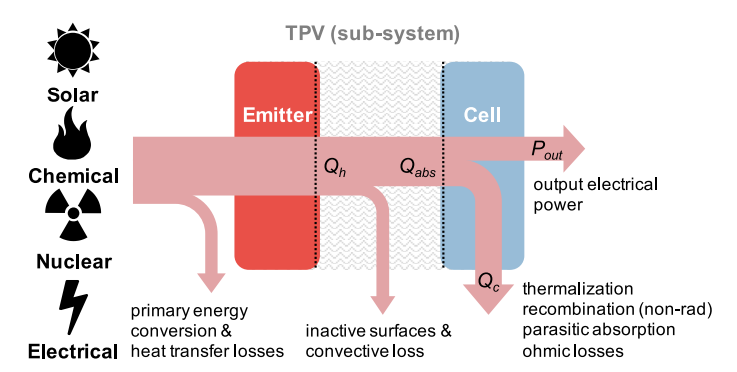
\includegraphics[width=0.7\textwidth]{figuras/TPV_Subsistema.png}
	\caption{Flujo de conversión de la energía térmica en energía eléctrica. \textit{Fuente: \cite{Present_Efficiencies_and_Future_Opportunities_in_Thermophotovoltaics}}}
	\label{fig:TPV_Subsistema}
\end{figure}
El emisor se encuentra a una alta temperatura lo cual produce que se transmite el calor en forma de radiación que al llegar a la célula es reflejada, transmitida o absorbida, la porción de radiación absorbida excita a los electrones produciendo un par electrón-hueco sí solo sí la energía del fotón absorbido es mayor que la energía de la banda energética de la célula, al conectar los terminales de la célula a una carga se produce una corriente que alimenta a la carga proporcional a la intensidad lumínica, aquellos fotones con energía menor a la banda energética son suprimidos o reflejados para disminuir el flujo de calor\cite{Present_Efficiencies_and_Future_Opportunities_in_Thermophotovoltaics}.\\\\
%%% INTERES EN LA TERMOFOTOVOLTAICA
La termofotovoltaica ha sido un campo de interés para aplicaciones militares, espaciales, generación de electricidad y recuperación de calor residual. Para la milicia de los Estados Unidos de América se han conducido varias investigaciones para la búsqueda de un generador eléctrico silencioso y portátil \cite{military_TPV}, cumpliéndose en 2004 40 años de investigación sin conseguirse potencias por encima de 500W \cite{military_TPV_40Years}. En aplicaciones espaciales es de interés por presentar beneficios en rendimiento para misiones cercanas al Sol y misiones en el espacio profundo porque los componentes más sensibles se encuentran resguardados de la dura radiación, siendo posible también el guardar energía en gravedad cero \cite{TPV_space_applications}. Para la recuperación de calor residual existe un gran interés porque la conversión de energía térmica a eléctrica es menor del 40\% en las plantas de generación de energía de combustibles fósiles convencionales, produciéndose una gran cantidad de pérdidas en forma de calor \cite{wasteHeat_TPV}.\\\\
%%% RESUMEN DE INVESTIGACIONES 
Todas estas áreas de interés ha provocado un aumento de las investigaciones en los sistemas de generación termo-fotovoltaicos, estudiándose la utilización de células multicapas, diferentes materiales de emisor para aumentar la potencia radiada, aplicación de capas finas en el emisor para el aumento de la potencia radiada\cite{doi:Near_field_ThinFilm}, aplicación de filtros \cite{multiLayerFilters} y capas reflectantes para la recuperación de fotones y disminución de calentamiento\cite{thermoionic_TPV_NF},la combinación con un TEC para aumentar la densidad de potencia y eficiencia total del sistema generador\cite{thermoionic_TPV_NF,progress_Thermoionic_TPV}, y la disminución del espacio entre emisor y célula para aprovechar los efectos de la radiación de campo cercano\cite{thermoionic_TPV_NF,modelEfficiency_NF_TPV,nf_TPV_Pillars_SiO2}.\\\\
%\cite{thermoionic_TPV_NF,modelEfficiency_NF_TPV,nf_TPV_Pillars_SiO2,NearField_200nm}
%%%  OTRA INVESTIGACIÓN 
Las investigaciones no se han limitado a estudiar células TPV de una o varias uniones p-n, sino también la utilización de células termofotovoltaicas interbandas en cascada (ICTPV) de banda energéticas comprendidas entre 0.2 y 0.5 eV que resulta en una eficiente colección de portadores foto-generados, donde la eficiencia máxima ($\eta_{max}$) y la diferencia de potencial en vacío ($V_{OC}$) es proporcional a el número de bandas (stages) hasta unos 0.691 V de $V_{OC}$ y uno 6.2\% $\eta_{max}$, pero genera una significante cantidad de energía térmica por la densidad de corriente oscura\cite{MultiEstados_Capas_TPVs}. Esta corriente se consigue disminuir al introducir una barrera entre las capas\cite{decreaseDarkCurrent}.\\\\
%%%  BACK SURFACE REFLECTOR AND FILTERS
Aún quedan por estudiar muchos materiales y disposiciones del emisor y de la célula, algo de alta importancia es el estudio de filtros y capas reflectantes porque permiten la re-utilización de los fotones no absorbidos, aumentando la eficiencia y evitando que se acabe calentando innecesariamente la célula. Las capas traseras reflectantes(BSR), principalmente hechas de oro, reducen las pérdidas de radiación por la absorción de la radiación de energía menor a la banda energética, permitiendo que la radiación vuelva al emisor \cite{nTPV_Review} (figura \ref{fig:TPV_BSR_altaEficiencia}).
\begin{figure}[H]
	\centering
		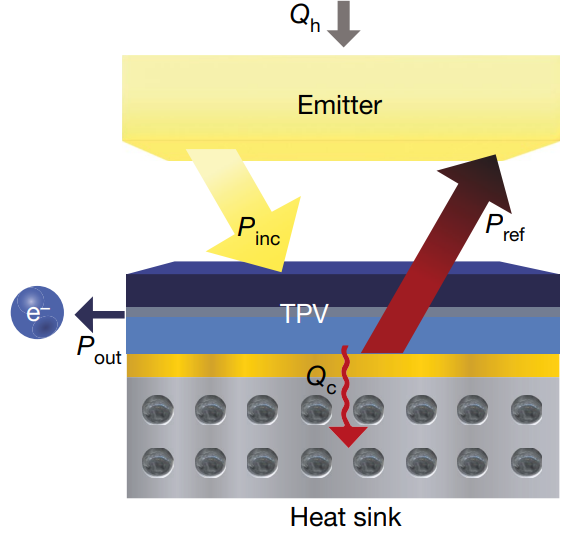
\includegraphics[width=0.6\textwidth]{figuras/TPV_40_BSR.png}
	\caption{Sistema generador TPV con BSR de oro, capa fina dorada entre la célula y el radiador). \textit{Fuente: \ref{thermophotovoltaic_40}}}
	\label{fig:TPV_BSR_altaEficiencia}
\end{figure}
Habitualmente estas capas se usan en las TPVs y TICs, como por ejemplo se usan en \cite{thermoionic_TPV_NF,modelEfficiency_NF_TPV,thermophotovoltaic_40}. Los filtros se utilizan para evitar la transmisión de radiación no deseada  la célula, consiguiéndose un aumento de la eficiencia del 45\% al 75\%, estos filtros pueden ser de una o múltiples capas que la rugosidad de la interfaz degrada seriamente la eficiencia, lo que se puede mejorar con una poca cantidad de capas\cite{multiLayerFilters}.\\\\
%% Ahora va las investigaciones y poco a poco intercalando entre ellas
%%% DIFERENTES CERAMICAS
En \cite{differentEmitterCeramics} se estudian diferentes combinaciones de cerámicas para el emisor de una TPV a 2000\textdegree C y célula a 400\textdegree C, observando los flujos espectrales de calor, la potencia total y el rendimiento, siendo la máxima potencia por metro cuadrado para el emisor de $B_4C$ con unos 7.45 $Wm^{-2}$ pero solo con una eficiencia del 11.74\%, a diferencia del BeO con una potencia de 3.19 $Wm^{-2}$ y un rendimiento del 24.69\%. Y se observa como el rendimiento disminuye al disminuir la separación entre emisor y célula para luego volver a aumentar.\\\\
%%%  COMBINACION DE TPV CON TIC
La razón por la cual se combinan los TICs y las TPVs es para aprovechar tanto los electrones como los fotones radiadios, aumentando la densidad de potencia de salida y mejorando el rendimiento de una TPV. Si se disminuye la separación entre el emisor común y la célula por debajo de la micra se pasa a tener efectos de campo cercano, aumentando la potencia producida. En \cite{thermoionic_TPV_NF} utilizan un dispositivo termofotovoltaico de campo cercano mejorado con termoiónico (nTiPV) con un emisor de Tungsteno con una capa de $LaB_6$ a unos 2000K, que mejora el rendimiento de una TPV de un 10\% de eficiencia a un 30\% y un aumento de densidad de potencia de unos 10$Wm^{-2}$ a unos 70 $Wm^{-2}$ (figura \ref{fig:PowerDensityVSEfficiency_nTiPV}), por el uso de una célula sin mallado, disminuyendo la resistencia en serie y las pérdidas por sombras, utilizando un BSR para reflectar los fotones de baja energía.\\
\begin{figure}[H]
	\centering
		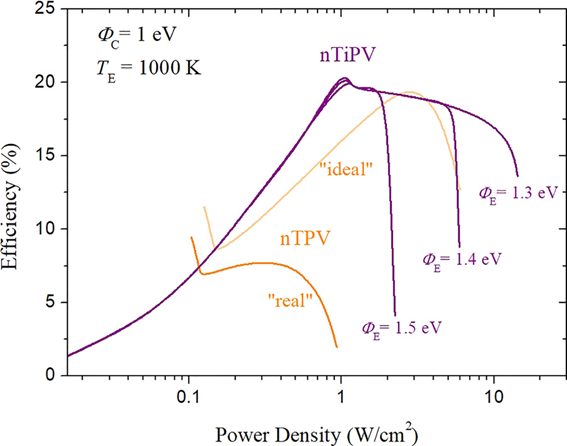
\includegraphics[height=7cm]{figuras/PowerDensityVSEfficiency_nTiPV.png}
	\caption{Relación entre densidad de potencia y eficiencia entre dispositivos nTPVs y nTiPVs. \textit{Fuente: \cite{thermoionic_TPV_NF}}}
	\label{fig:PowerDensityVSEfficiency_nTiPV}
\end{figure}

%%% CAMPO CERCANO
Los dispositivos TPV que aprovecha el efecto de campo cercano se denotan como dispositivos NFTPV, NF-TPV o nTPV, esto en combinación con el objetivo de disminuir la contaminación, aprovechar la energía desperdiciada en forma de calor y utilizar baterías más baratas con gran almacenamiento de energía ha impulsado bastante las investigaciones al respecto de la tecnología NF-TPV. Siendo el aumento de la eficiencia para igualar a la actual de campo lejano de 40\% \cite{thermophotovoltaic_40} un objetivo interesante, en \cite{modelEfficiency_NF_TPV} se modeló la eficiencia de un NF-TPV basado en InAs con emisor a  700K y radiador de la célula a 300K, alcanzándose unas eficiencia del 17\% siendo la separación de 200nm y notándose que a menores temperaturas y mayores distancias se obtiene menos potencia, y notando que al aumentar la temperatura el pico de potencia se desplaza a menores longitudes de onda.\\

%%% ECUACIONES
Dado que los costes de fabricación para el testeo pueden llegar a ser caros se utilizan modelos matemáticos para simular, siendo uno muy útil el presentado en \cite{nfTPV_equations} que proporciona varias ecuaciones para calcular la potencia radiada para varios grosores de emisor y receptor de una sola capa cada uno, siendo el de mayor utilidad el de capa gruesa que proporciona de una manera sencilla el cálculo de la potencia en un rango de longitudes de onda conociendo la función dieléctrica compleja de los materiales.\\

%%% FRECUENCIA DE RESONANCIA Y CAPAS FINAS PARA AUMENTO DE ENERGIA
Una ventaja que presenta los NF-TPV es la frecuencia de resonancia ($\omega_{res}$), que produce una mejora o aumento del flujo radiado a dicha frecuencia. En \cite{doi:Near_field_ThinFilm} utilizan una lámina fina de SiC y otra gruesa, obteniendo que al aumentar el grosor de la capa disminuye la potencia en la $\omega_{res}$ pero aumenta para el resto de frecuencias, siendo a partir de los 100nm de grosor la misma potencia radiativa que la lámina gruesa. Para mantener las distancias tan cortas es necesario un mecanismo, siendo lo más sencillo el uso de pilares de algún material cerámico por sus propiedades térmicas, como se presenta en \cite{NearField200} que estudia la transferencia de calor entre dos placas de Si separadas 200nm por vacío y utilizando espaciadores de SiO2 y prismáticos de base circular de 1 $\mu m$ de diámetro fabricados con fotolitografía ultravioleta, obteniéndose que el coeficiente radiativo de transferencia de calor aumenta con la disminución de la separación entre emisor y célula, y aumenta con la temperatura.\\

%%% RESISTENCIAS DE CONTACTO
También hay que tomar en cuenta la existencia de las resistencias de contacto entre cada interfaz, teniendo una gran importancia en \cite{nf_TPV_Pillars_SiO2} que estudia la radiación por campo cercano entre dos placas de cuarzo con pilares de pirámides truncadas de $SiO_2$ que están depositados sobre el substrato inferior, descubriéndose que la resistencia de contacto es mucho mayor que la geométrica del pilar, por lo tanto, es de gran importancia para disminuir las pérdidas por conducción.\\


\section{Transmisión de calor}
El calor es una forma de energía que se propaga entre distintos medios de tres formas distintas, por convección, radiación y conducción.
\subsection{Convección}
La transmisión de calor por convección se produce por la conducción de la energía cuando el fluido entra en contacto con el sólido y luego el transporte de la energía mediante el movimiento del fluido, pudiendo ser natural o forzada. La diferencia entre la convección natural y la forzada es la fuente de movimiento del fluido, en la convección forzada el movimiento del fluido es producido por una fuente externa, como un ventilador o una bomba, en la convección natural el fluido se mueve por las diferencias en densidades por la variación de la temperatura de partes del fluido.\\
\subsection{Radiación}
La radiación es la transmisión de energía térmica en forma de ondas electromagnéticas o fotones a través del vacío o un medio material proporcional a la temperatura del cuerpo del emisor. Cuando las ondas electromagnéticas inciden sobre la superficie de un material parte de ella es absorbida, otra parte reflejada y el resto se transmite internamente en el material, variando las proporciones de dichas cantidades según el material y la longitud de onda de la radiación. Existe dos flujos de radiación conocidos, el flujo de propagación o campo lejano y el flujo evanescente o campo cercano que excede los valores predichos por la Ley de Planck del cuerpo negro.\\

\subsubsection{Radiación propagación o campo lejano}
La radiación de campo lejano cumple la regla de Planck sobre la emitancia monocromática de un cuerpo negro (${E_{\lambda}}^{bb}(T)$) (ecuación \ref{eq:ecuacionPlanck}), cuyo valor total cumple con la Ley de Stefan Boltzmann (ecuación \ref{eq:leyDeStefanBoltzmann}) y el valor máximo cumple con la Ley de Wien, $\lambda_{max}\cdot T=2.896\cdot 10^3 \mu m\cdot K$, donde la temperatura (T) está en grados Kelvin.

\begin{equation}
{E_\lambda}^{bb}\left( T \right) = \dfrac{c_1\cdot \lambda^{-5}}{e^{\frac{c_2}{\lambda \cdot T}}-1}
\label{eq:ecuacionPlanck}
\end{equation}
\begin{equation}
{E}^{bb}\left( T \right)=\sigma \cdot T^4 \qquad \Longleftrightarrow \qquad \sigma = 5.67\cdot 10^{-8} \dfrac{W}{m^2 K^4}
\label{eq:leyDeStefanBoltzmann}
\end{equation}

 Pero las ecuaciones anteriores solo aplica para la radiación total emitida pero no la transferida entre dos superficies, siendo el caso más sencillo el de dos superficies planas, paralelas entre sí y de área infinita o mucho mayor que la distancia que las separa, donde la transferencia de calor entre ambas superficies consideradas como cuerpos grises se puede modelar como:
\begin{equation}
\frac{\Phi}{S}=\frac{\sigma \left( T_1^4 -T_2^4 \right)}{1/\epsilon_1 +1/\epsilon_2 -1}
\label{eq:flujoCalorSuperficiesGrises}
\end{equation}
Donde $\epsilon_i$ es la emisividad monocromática, es decir, el cociente de la emisividad del cuerpo respecto a la del cuerpo negro, cuyo vaor es constante por ser considerados las superficies como cuerpos grises.\\

Para la radiación de propagación en campo cercano se denota se resuelve de otra manera, que en el caso más sencillo el emisor y el receptor son cuerpos planos y gruesos (figura \ref{fig:campoCercanoEquation1}), la ecuación que modela el flujo de calor por frecuencia de un emisor (nº1) a un receptor (nº3) separados por el vacío (nº2) es \cite{nfTPV_equations}:

\begin{equation}
q_{w,abs}^{prop}=\dfrac{\Theta \left( \omega,T_1 \right)}{4 \pi^2}\times \int^{k_\upsilon}_{0} k_\rho d k_\rho \sum_{\gamma=TE,TM}\dfrac{\left( 1- \left| r_{21}^\gamma \right|^2\right) \left( 1-  \left| r_{23}^\gamma \right|^2 \right)}{\left| 1- r_{21}^\gamma r_{23}^\gamma e^{2ik_{z2}d_{c}} \right|^2}
\label{eq:flujoPropNF}
\end{equation}
Donde $\Theta \left( \omega,T_i \right)$ es la energía media de un oscilador de Planck para una frecuencia y temperatura dada, $r_{i,j}^\gamma$ es el coeficiente de reflexión de Fresnel de la interfaz entre el cuerpo i y el cuerpo j en estado polarizado $\gamma$, TE son las ondas eléctricas transversales y TM son las ondas magnéticas transversales, i es la constante compleja $\sqrt{-1}$, $d_c$ es la separación entre las capas y $k_\rho$ es el vector de onda de la onda primaria \cite{nfTPV_fullEquations}.\\
\begin{figure}[H]
	\centering
		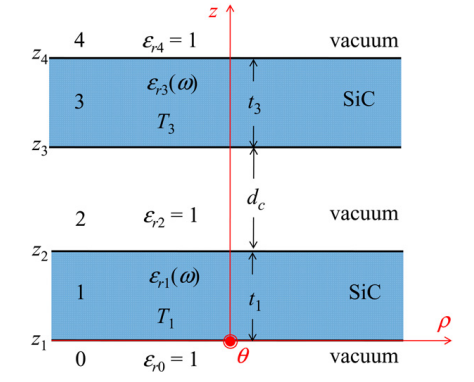
\includegraphics[height=7cm]{figuras/campoCercanoEquation1.png}
	\caption{Esquemático de la representación geométrica para el flujo entre dos cuerpos separados por vacío. \textit{Fuente: \cite{nfTPV_equations}}}
	\label{fig:campoCercanoEquation1}
\end{figure}
La ecuación \ref{eq:flujoPropNF} es para dos placas gruesas separadas por un vacío y rodeadas por vacío, se obtiene de las ecuaciones presentadas en \cite{nfTPV_fullEquations}, donde se presenta las ecuaciones para la radiación de campo cercano de sistemas multicapa y un método numérico para solucionar las ecuaciones.

\subsubsection{Radiación evanescente o campo cercano}
La radiación evanescente se transmite distancias muy pequeñas la cual puede ser aprovechada para la recuperación del calor residual, introduciéndose un algoritmo general para el análisis de un sistema unidimensional multi-capa basado en las funciones de dyadic Green y la amplitud para cada capa es calculada con una matriz de dispersión \cite{nfTPV_fullEquations}, obteniéndose para el caso de dos capas gruesas separadas por vacío una distancia $d_c$, el flujo de la radiación evanescente \cite{nfTPV_equations} como :
\begin{equation}
q_{\omega,abs}^{evan}=\dfrac{\Theta \left( \omega,T_1 \right)}{\pi^2}\times \int^{\infty}_{k_\upsilon}k_\rho d k_\rho e^{-2k_{z2}'' d_c} \sum_{\gamma=TE,TM} \dfrac{Im\left( r_{21}^\gamma \right)Im\left( r_{23}^\gamma \right)}{\left| 1- r_{21}^\gamma r_{23}^\gamma e^{2ik_{z2}d_{c}} \right|^2}
\label{eq:flujoEvasNF}
\end{equation}

Siendo $Im\left(r_{i,j}^\gamma \right)$ el término imaginario del coeficiente Fresnel de la interfaz entre el cuerpo i y el cuerpo j en estado polarizado $\gamma$. La componente $e^{-2k_{z2}'' d_c}$ representa de manera explícita la caída exponencial del flujo con la distancia de separación. Una mejor representación del efecto de la radiación evanescente se puede observar en la figura \ref{fig:graficaDiff_dc_fullEqu}, donde a partir de cierta distancia de separación se supera el flujo de un cuerpo negro. Y se observa en la figura \ref{fig:graficaDiff_t_fullEqu} como a partir de las 100$\mu m$ de grosor del emisor se puede considerar como una placa gruesa \cite{nfTPV_fullEquations}.

\begin{figure}
\centering
\begin{subfigure}[b]{0.48\textwidth}
	\centering
		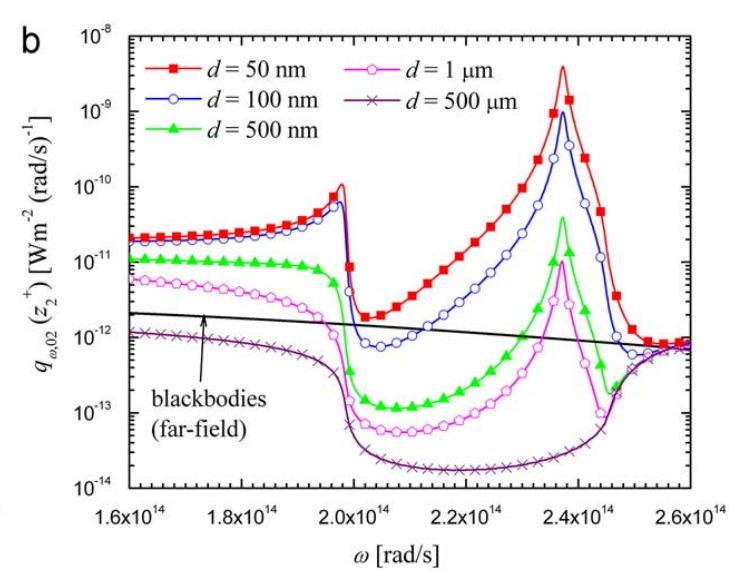
\includegraphics[width=\textwidth]{figuras/graficaDiff_dc_fullEqu.png}
		\caption{flujo de radiación monocromática variando la distancia de separación d}
	\label{fig:graficaDiff_dc_fullEqu}
\end{subfigure}
\begin{subfigure}[b]{0.48\textwidth}
	\centering
		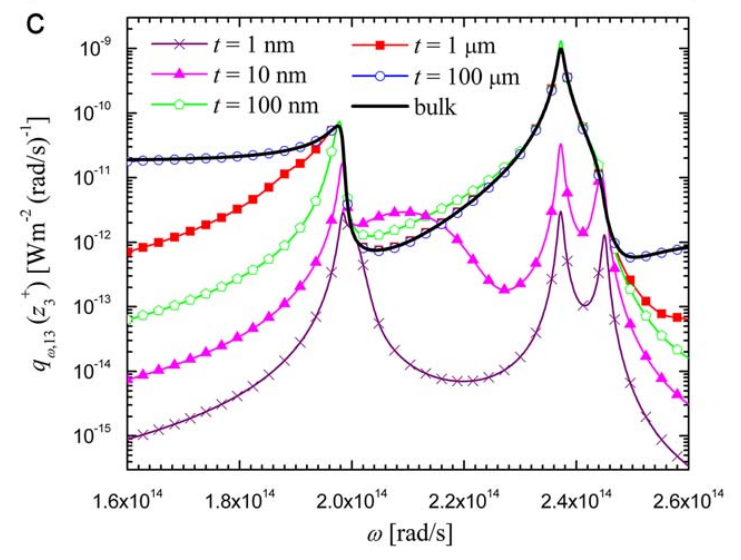
\includegraphics[width=\textwidth]{figuras/graficaDiff_t_fullEqu.png}
		\caption{flujo de radiación monocromática variando el grosor (t) del emisor}
	\label{fig:graficaDiff_t_fullEqu}
\end{subfigure}
\caption[Flujos de radiación monocromática por variación de grosor de emisor y variación de distancia]{(\subref{fig:graficaDiff_dc_fullEqu}) Flujo de la radiación monocromática entre dos capas gruesas de cBN a 300K y 0K separadas por vació a una distancia d, y comparados con las predicciones de dos cuerpos negros en el régimen del campo lejano. (\subref{fig:graficaDiff_t_fullEqu})Flujo de la radiación monocromática entre un emisor de grosor (t) variable a 300K y un receptor grueso a 0K, ambos de cBN y separados por una distancia de 100nm en el vacío. \textit{Fuente: \cite{nfTPV_fullEquations}}}%
\label{fig:graficas_fullEqu}%
\end{figure}

\subsection{Conducción}
La transmisión de calor por conducción se dá a través de uno o varios cuerpos, producido por la diferencia de temperatura entre las caras opuestas del conjunto o cuando dos o más objetos a diferentes temperaturas entran en contacto. De manera genérica la conducción térmica se modela como $P_{cond}={\bigtriangleup T}/{R} $, siendo $R$ la resistencia térmica del sistema.
Para un solo material, la resistencia térmica se modela como $R = l/{\left(A\cdot h\right)}$, donde $l$ es la longitud del material, $A$ es la superficie y $h$ es la conductividad térmica del material. Para varios materiales colocados en serie, es decir, el flujo de calor que los atraviesa es el mismo para todos, la resistencia de conducción se define como la sumatoria de todas las resistencias de cada material($R=\sum R_i$).\\

La superficie de contacto entre cada material se le conoce como interfaz, la cual en la realidad no es perfecta y provoca una caída de temperatura la cual se modela como una resistencia térmica llamada resistencia de contacto ($R_c$). La resistencia de contacto depende de muchos parámetros como la rugosidad de cada superficie, la presión, la temperatura, las conductividades térmicas de los materiales involucrados, los tipos de materiales, entre otros, esto provoca que sea muy difícil de obtener un modelo de la misma para una simulación.\\

En \cite{experimental_Rc_SS} comparan la desviación entre los experimentos y la teoría de la resistencia de contacto entre varios materiales, siguiendo el modelo teórico utilizado para la zona plástica una ecuación simplificada, que para dos aceros inoxidables 304 la diferencia entre experimentación y teoría disminuye con el aumento de la presión. Dichas ecuaciones teóricas que modelan la variación de la resistencia de contacto con la presión son:

\begin{subequations}
\begin{equation}
\dfrac{h_c\sigma}{k_sm}=1.25\left(\dfrac{P}{H_c}\right)^{0.95}
\label{eq:correlacionCooperSimplificadaYovanovich}
\end{equation}
\begin{equation}
\dfrac{P}{H_c}=\left[ \dfrac{P}{c_1\left(1.62\sigma/m\right)^{c_2}} \right]^{\frac{1}{2+0.071c_2}}
\label{eq:modeloYovanovich}
\end{equation}
\label{eqs:ecuacionesRcYovanovich}
\end{subequations}

Donde los valores de las constantes $c_1$ es 10.6 GPa y $c_2$ es -0.40, y donde $\sigma$ es la combinación RMS de la rugosidad de ambas superficies de los materiales con $\sigma_i$ siendo la rugosidad de la superficie $i$ (ecuación \ref{eq:mRMS}), $m$ es la combinación RMS de la media absoluta de la pendiente de la rugosidad con $m_i$ siendo la media de la pendiente absoluta de la rugosidad de la superficie $i$ (ecuación \ref{eq:sigmaRMS}), $H_c$ es la micro-dureza Vickers del material más duro y P es la presión aplicada \cite{experimental_Rc_SS}.

\begin{subequations}
\begin{equation}
m=\sqrt{m_1^2+m_2^2}
\label{eq:mRMS}
\end{equation}
\begin{equation}
\sigma=\sqrt{\sigma_1^2+\sigma_2^2}
\label{eq:sigmaRMS}
\end{equation}
\label{eqs:RMS}
\end{subequations}